
\chapter{Tehtävä 1 \label{chap:Teht=0000E4v=0000E4-1}}

Tehtävänä oli malintaa kolme matopelin tapausta käyttötapauskaavioilla
\section{Mato pelin mallinnus}

\label{Madon liikkuminen}

Madon liikkuminen kehyksessä tapahtuu niin että, käyttäjä antaa suunnan mihin liikutaan ja mato liikkuu jokaisella 
tickillä vähäsen siihen suuntaan kunnes pelaaja vaihtaa suuntaa. Pelaaja ohjaa madon päätä ja madon häntä tulee perässä
niin että jokainen hännän osa saa koordinaateiksi sitä edeltävän osan vanhan paikan.

\begin{figure}
\centering \includegraphics[width=0.5\textwidth]{kuvat/SnakeGame1}
\label{Liikkuminen} 
\end{figure}

\label{Evään syönti}
Kun madon pään koordinaatit ovat samat kuin evään, eväs syödään eli poistetaan kehyksestä. Mato saa pisteitä eväältä ja sen häntä kasvaa yhden pykälän. Uusi eväs asetetaan jonnekin kehykseen. 

\begin{figure}
\centering 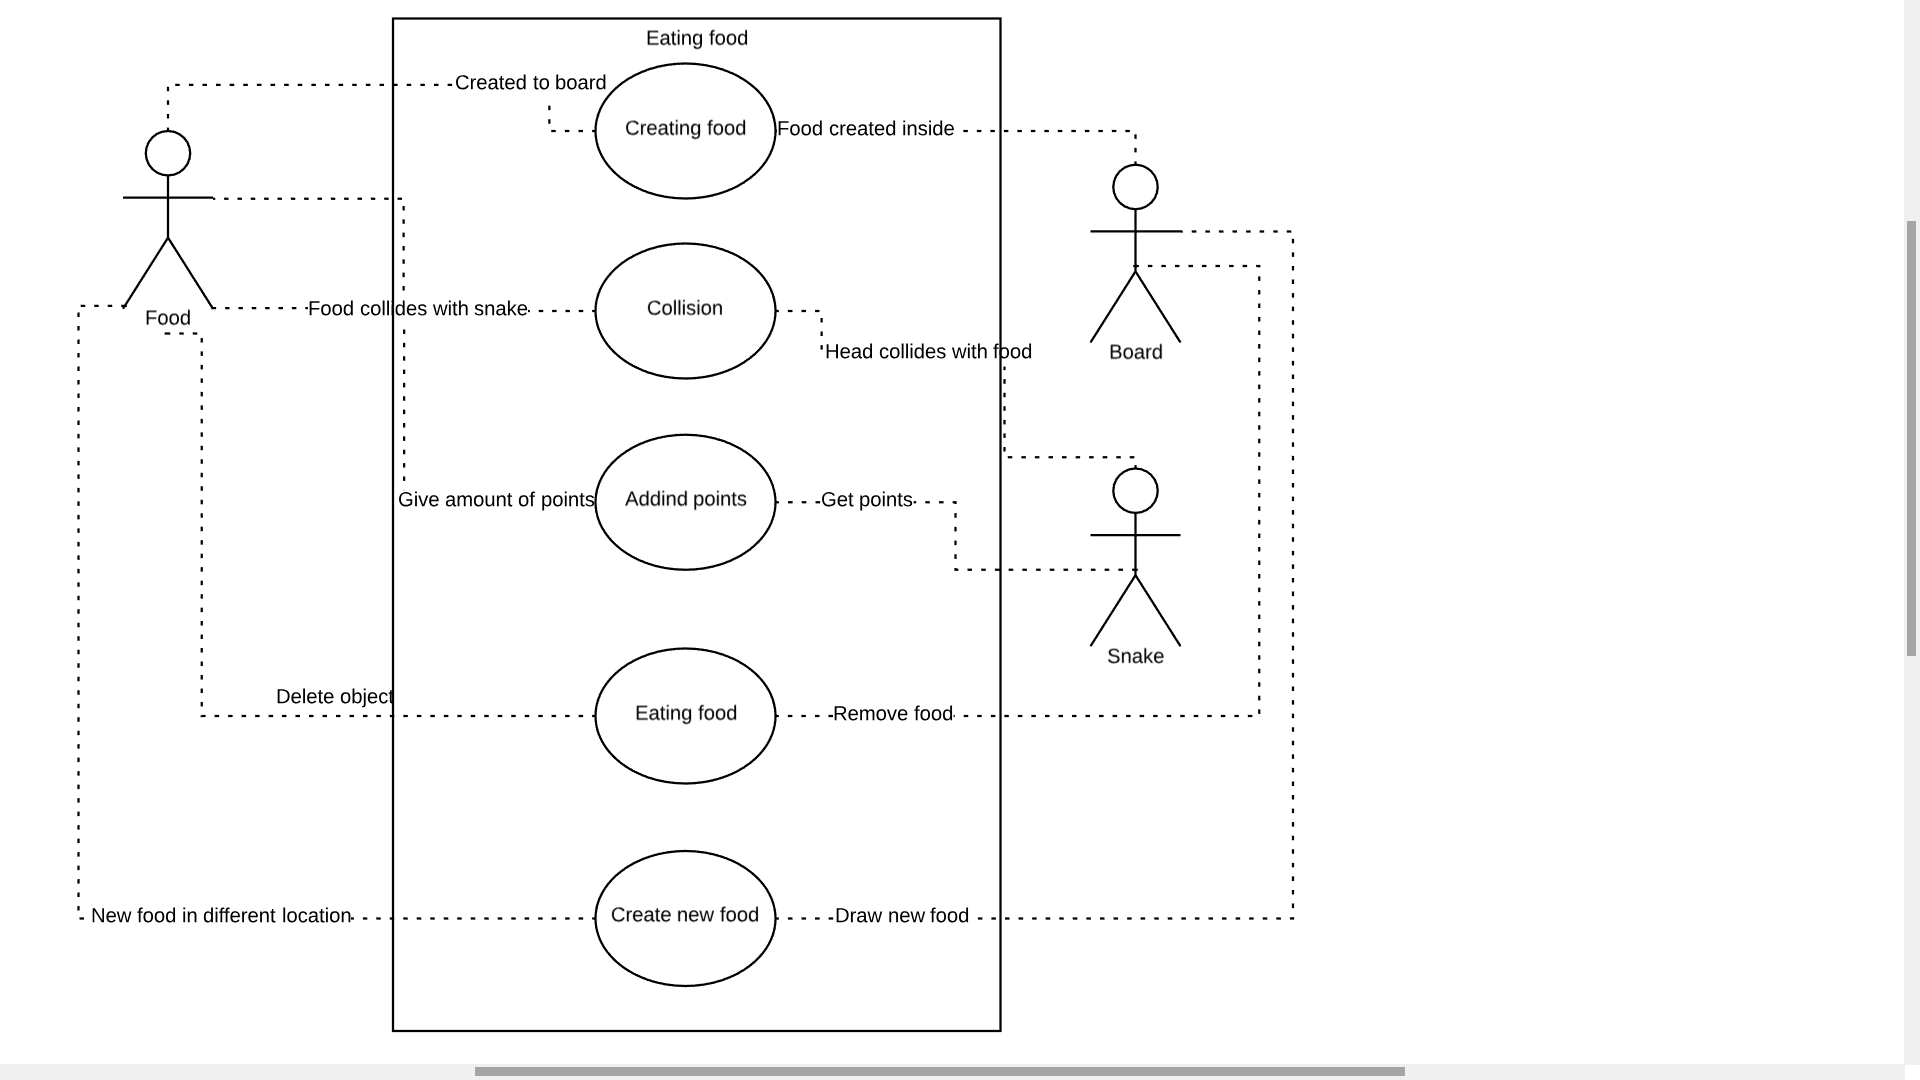
\includegraphics[width=0.5\textwidth]{kuvat/SnakeGame2}
\label{Syönti} 
\end{figure}

\label{Törmäys}
Jos mato osuu kehyksen seinään se menettää pituutta ja pysähtyy kunnes sille annetaan uusi suunta. 
\begin{figure}
\centering 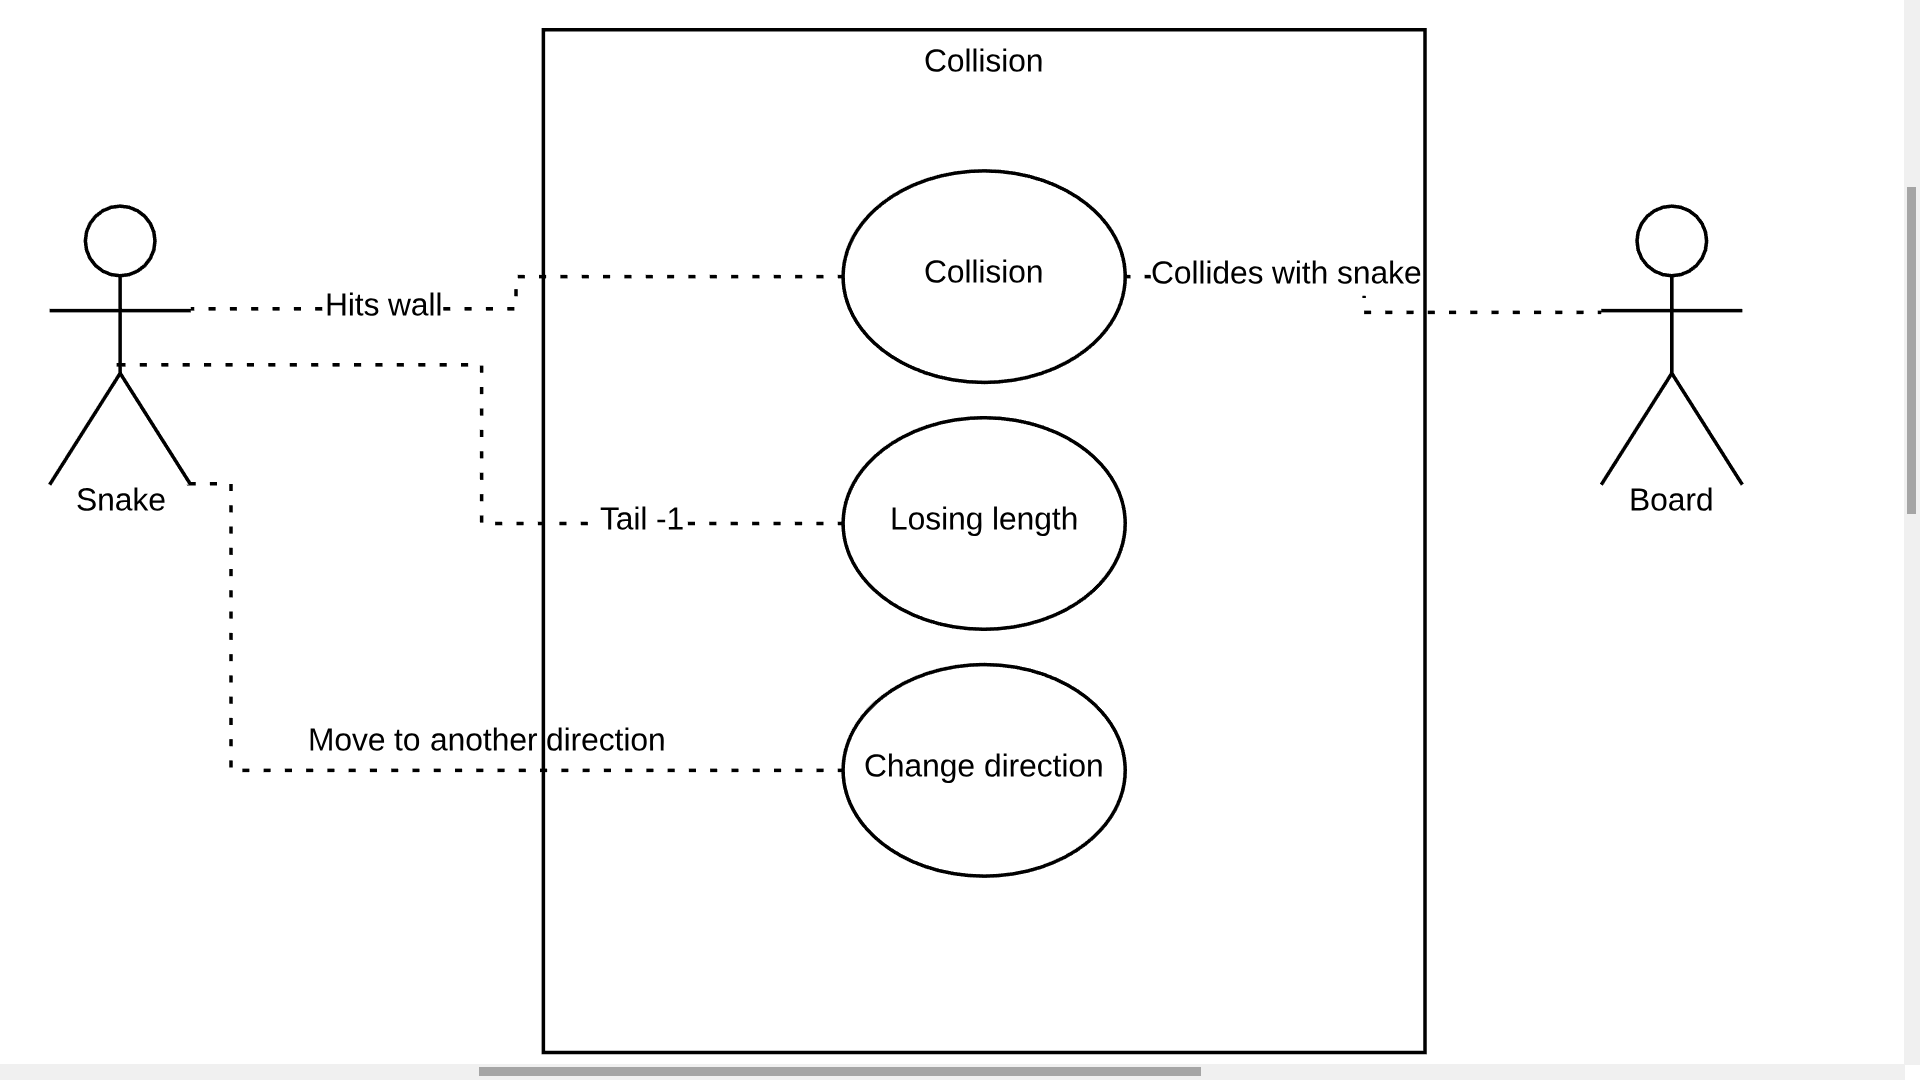
\includegraphics[width=0.5\textwidth]{kuvat/SnakeGame3}
\label{törmäysSeinään} 
\end{figure}




- Janina Kuosmanen (516580)
